\chapter{Problem Presentation}
Given the premises presented in the previous chapters, our work mainly focused on two open issues regarding both the dictionary learning and the graph learning problem. The starting point were the works of Dorina Thanou -  regarding the dictionary learning approach for graph signals - and the work of Hermina Petric Maretic - regarding the graph learning approach.\\
In the related work, Thanou et al. proposed a learning algorithm which was able to retrieve the kernel functions for a certain dictionary, alternatively optimizing over the kernel coefficients $\alpha$ and the sparsity matrix $X$, while Maretic et al. started from the complementary assumption that the entities known in their case where exactly the kernel coefficients, while they alternatively optimized over the sparsity matrix and the graph weight matrix.

\section{State of the art}
There has already been a discrete amount of work around graph inference for signals that are expected to be smooth on the graph.  In \cite{Dong2016} Dong et al. addressed the problem adopting a factor analysis model for graph signals and imposing a Gaussian probabilistic prior on the independent variables which model the signal. Their results showed that smoothness property of a graph signal is favoured by the efficient representation obtained through these priors. In particular, in the algorithm they presented they deployed the use of $l^1$ and Frobenius norm, the former is expressed by a constraint on the Trace of the Laplacian, and eventually accounts for a sparsity term, while the latter is added as a penalty term in the objective function in order to control the distribution of the off-diagonal entries in L.

At the same time, in \cite{Kalofolias2016} Kalofolias proposes another framework to learn a graph structure under the smoothness assumption. They also use the minimization of the trace term for the Laplacian matrix, clinching that the minimizations of it brings to naturally sparse solutions.

However, this assumption is not always exhaustively descriptive of the real problem we are considering, so we might want to add other reinforcements to the priors in order to better describe the situation. For example, we could imagine a real world network to show a localized behavior or a more organized one having a certain pattern repeating over the graph. In \cite{Maretic2017}, this was an assumption for the signal, bringing it to be a sparse combination of a small number of atoms in a polynomial graph dictionary. This in the end was creating atoms localized in every node on the graph, repeating the same pattern over it with respect to every node as a source, in the same way it is described in \cite{Thanou2014}. However Maretic's work is limited by the fact that, as we already mentioned, it assumes the kernels to be know functions while it concentrates only on the graph dictionary and thus fixing the spectral behavior of the atoms.

\section{Problem structure}
As previously mentioned, this work deals with the general class of signals that can be represented in a sparse way through atoms of a polynomial dictionary \cite{Thanou2014}, such that it can give a natural segregation of each signal into localised components, as shown in \autoref{fig:components}. The figure shows how each of these components derive from one atom, which is directly dependent of the graph dictionary. This is well explained if, for polynomial kernels of degree k, we see our atoms as an entity spanning only the k-hop distance from the node that represents the center of the atom (source), as we will describe in the next section.

\begin{figure}
\centering
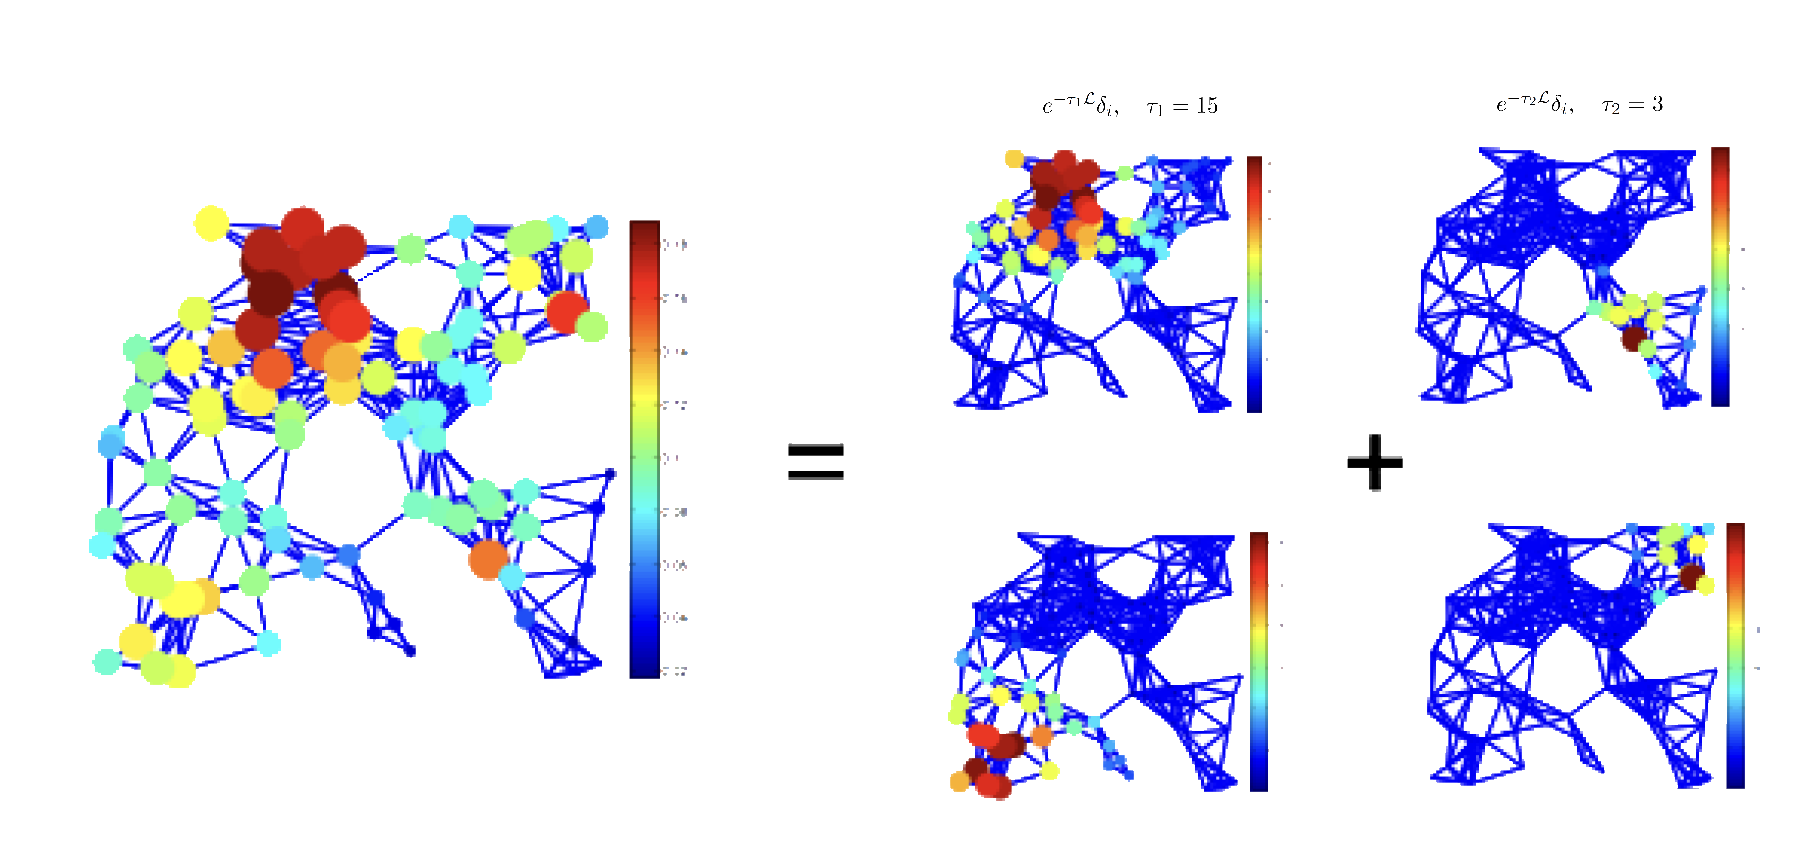
\includegraphics[width = .8\textwidth]{SignalDecomposition.png}
\caption{Example of signal decomposition using the polynomial dictionary}
\label{fig:components}
\end{figure}

In continuity with the prior work, here we assume the sources of our atoms to be unknown and not necessarily the same for all the different generated parts of the signal. This means, in mathematical terms, assuming that we do not know \textit{a priori} the position, in the columns of the sparsity matrix $X$, of the non-zero entries that indicate which are the nodes acting as sources for the atoms.

Closely related to the segregation assumption then, is the fact that we could imagine our signal as having a sort of community structure. This means that the graph can be clustered into communities that are poorly related among themselves when talking about the signal variation, thus imagining very different node signals to be sufficiently distant, and so, being part of separated communities.

% Another strictly related assumption, is that the graph has a strong community structure, meaning that the graph can be separated into communities which are poorly related among themselves, but hold strong connections inside them. These two assumptions are somewhat exchangeable, such that an interesting aspect to develop in the future could be reducing one of them.

\subsection{The translation operator and the smoothness priors}
To better describe the structure of our dictionary, we start recalling that in \autoref{sec:graph laplacian} we introduced the Laplacian operator as $L = D - W$ and here we focus on a modified version of this operator, that is the \textit{normalized Laplacian} $\mathcal{L} = D^{-\frac{1}{2}}LD^{-\frac{1}{2}}$. The normalized Laplacian is also a real symmetric and positive semidefinite matrix, with a complete set of orthonormal eigenvectors $\textbf{$\chi$} = [\chi_0,\chi_1,\dots,\chi_{N-1}]$ and associated non negative eigenvalues $\sigma(\mathcal{L}) := \{ 0 = \lambda_0,\lambda_1,\dots,\lambda_{N-1} \leq 2 \}$ (where the upper bound 2 comes from the normalization).
The normalized Laplacian eigenvectors are Fourier basis, this bringing any function $y$ defined on the vertices of the graph to be represented in his Fourier transform version $\hat{y}$ at frequency $\lambda_l$ as:
\begin{equation}
\hat{y}(\lambda_l) = \langle y, \chi_l \rangle = \sum_{n=1}^{N} y(n)\chi_l^{*}(n)
\end{equation}
and its relative inverse transform to be:
\begin{equation}
y(n) = \sum_{l=0}^{N-1} \hat{y}(\lambda_l)\chi_l(n), \quad \forall n \in \mathcal{V}
\end{equation}
This transform plays a major role not only in the harmonic analysis, but also in defining the signal translation onto a graph, which actually is the main transformation we are interested in when we try to construct a graph dictionary. It is worth to notice here that in the classical signal processing field the translation operator is defined through the change of variable $(T_n f)(t) := f(t-n)$, but when it comes to graph signal processing, this concept looses meaning since there is no significate to $f(\circ - n)$ in the graph environment. However, from transform theory we can recall that the classical translation operator $T_n$ can also be seen as a convolution with a Kronecker delta $\delta$ centered in $n$\cite{Shuman2013} \cite{Thanou2014}:
\begin{equation}
T_n g = \sqrt{N}(g * \delta_n) = \sqrt{N}\sum_{l=0}^{N-1}\hat{g}(\lambda_l)\chi_l^{*}(n)\chi_l \quad .
\label{eq:translation}
\end{equation}

This leads to think about \autoref{eq:translation} as an operator acting on the kernel $g(\cdot)$ directly defined in the spectral domain and from which we can obtain the effective translation to kernel $n$ through inverse graph Fourier transform. Moreover the term $\sqrt{N}$ in the \autoref{eq:translation} is a guarantee for the translation operator to preserve the mean value of the signal.\\

Now, in all of this we can assume the signal to have a smooth support as the one described in \autoref{ch:smoothness}; this prior is carried by the kernel entity  $g(\cdot)$ and can be seen as a measure to control the localization of $T_n g$ centered at vertex $n$ (meaning that the magnitude ($T_n g$)(i) of the translated kernel at vertex $i$ decays with the increasing distance from the center of the kernel). We can thus compose our atoms $T_n g$ as smooth entities, coming from the assumption that the kernel function in \autoref{eq:translation} is a smooth polynomial function of degree K:
\begin{equation}
\hat{g}(\lambda_l) = \sum_{k=0}^{K} \alpha_k\lambda_l^k, \quad l = 0,\dots,N-1
\end{equation}
From this fact, we can so obtain a global expression for a translation operator as:
\begin{align}
T_n g & = \sqrt{N}(g * \delta_n) = \sqrt{N}\sum_{l=0}^{N-1}\sum_{k=0}^{K}\alpha_k\lambda_l^k\chi_l^*(n)\chi_l \notag\\
&= \sqrt{N}\sum_{k=0}^{K}\alpha_k\sum_{l=0}^{N-1}\lambda_l^k\chi_l^*(n)\chi_l = \sqrt{N}\sum_{k=0}^{K}\alpha_k (\mathcal{L}^k)_n
\end{align}
where $(\mathcal{L})_n$ represents the $n^{th}$ column of the $k^{th}$ power of the Laplacian matrix $\mathcal{L}^k$. The final concatenation of $N$ such columns brings us to generate a set of $N$ atoms, corresponding to the columns of
\begin{equation}
Tg = \sqrt{N}\hat{g}(\mathcal{L}) = \sqrt{N}\chi \hat{g}(\Lambda)\chi^T = \sqrt{N}\sum_{k=0}^{K}\alpha_k\mathcal{L}^k
\label{eq:tg}
\end{equation}
Where the quantity $\Lambda$ corresponds to the diagonal matrix of the eigenvalues in such a way that the following relation holds: $\mathcal{L} = \rchi \Lambda \rchi^T$ \cite{Dong2016}. This brief section has the intrinsic meaning that if the kernel $g(\cdot)$ is a polynomial of degree $K$, then the translation operator is $0$ in all the vertices $i$ that are more than $K$ hops far away from the center vertex $n$, which means that the vertex domain support of the translated vertex is contained in a sphere of radius $K$ and center in $n$ and its magnitude decades with the increasing distance from $n$ to $i$.
In \autoref{fig:minnesota} there is an example of an atom translation in three different ways.

\begin{figure}[tb]
  \centering
  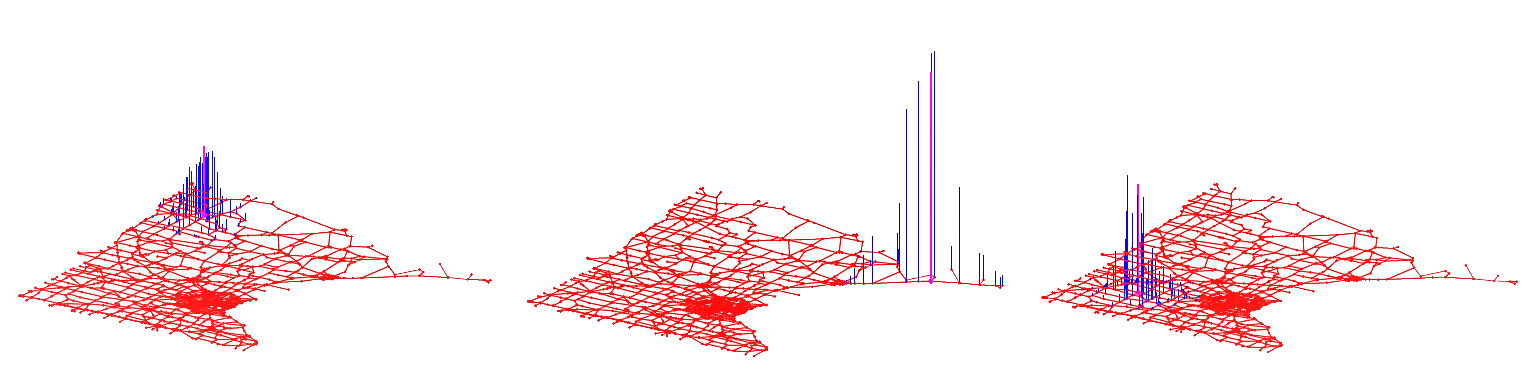
\includegraphics[width = \textwidth]{MinnesotaTranslation.png}
  \caption{Example of graph signal translation: translation for $T_{200}g$ (a), $T_{1000}g$ (b) and $T_{2000}g$ (c)}
  \label{fig:minnesota}
\end{figure}

\subsection{Dictionary learning section}
\label{sec:2implementations}
Gives the previous background, this part of the learning problem mainly tries to identify useful criteria for the way each kernel function spreads over the surrounding nodes. If, in fact, we were able to define the behavior of an atom inside its surroundings, we could use this information to sum up the description of a graph's portion in a more accurate way.
% This accomplishment, moreover, could give a further method to relate the general structure of a graph (seen as separable into communities) to the inner one, thus
% : we would like, for example, to establish a criteria to cluster a graph signal into several so called \textit{supernodes} connected among themselves and to relate the \textit{coarsened graph} so obtained the inner structure of each \textit{supernode}.

Since experimental description of real-life graph structures gives us reasons to believe that they tend to rely on smooth patterns (and so, low frequencies), assuming a certain kernels structure could be a way to relate the manifold macrostructure with its inner structure. From this, we arrive to the main assumption in our work, which is kernels smoothness: what we wish is that our atoms were representative of the portion of the graph they are covering, so that they should spread with non trivial values over all nodes of the subgraph. For this reason we constrained our dictionary kernels in such a way that they have mostly smooth support in the surroundings of the source node. To  be precise, this concept is something different form the smoothness assumption we widely examined in the previous sections: it adds some more information strictly related to the behavior of the kernel itself. In fact, if we learned a smaller order polynomial with constraints in high frequencies, we would not have a large spread of our atoms, things we want to have so that our atoms can represent a large portion of the graph.

To have this new smoothness constraint we look at the kernel polynomial:
\begin{equation}
g(\lambda) = \sum_{k=0}^{K}\alpha_k \lambda_k
\end{equation}
and we try to constraint the roots to correspond to the highest eigenvalues.\\
This would change the expression of the kernel and turn our learning problem into a simpler one.

In order to include this new smoothness notion we could go along two different paths:
\begin{itemize}
\item We could add this information into the objective function;
\item Or we could add the information to the constraints;
\end{itemize}

\subsubsection{Smoothness prior in the objective function}
In the first case the problem becomes trying to learn a smaller number of coefficients in the kernel function:
\begin{align}
g(\lambda) &= h(\lambda)(\lambda - \lambda_N)(\lambda - \lambda_{N-1})\cdot \dots \cdot (\lambda - \lambda_{N-M+1}) \label{eq:polynom}\\
where \qquad h(\lambda) &= \sum_{n=0}^{K-M}\gamma_n\lambda^{n} \notag
\end{align}

With this statement as start, we could try to give a first formulation of our problem, where we try to also include the fact that the atoms in the dictionary are actually coming from a graph dictionary. In fact, if we assumed these atoms to be only vectors describing the signal, we would keep this part separated from the graph notion.

With the previous formula we can thus arrive to a dictionary problem of this type:
\begin{align}
\underset{{\gamma_0,\dots,\gamma_{K-M}X}}{\argmin} \quad& ||Y - \mathcal{D}X||^2_F + \alpha||\mathcal{D}||_1 \label{eq:opt}\\
with \qquad g(\lambda) &= h(\lambda)(\lambda - \lambda_N)(\lambda - \lambda_{N-1})\cdot \dots \cdot (\lambda - \lambda_{N-M+1}) \notag\\
h(\lambda) &= \sum_{n=0}^{K-M}\gamma_n\lambda^{n} \notag\\
\mathcal{D}_i &= [g(L_i)]_{\text{source}_i} \notag\\
0 &\leq g(\lambda) \leq c \label{eq:ProblemPres1}\\
(c-\epsilon)I &\preceq \sum_{s=1}^{S}\mathcal{D}_s \preceq (c+\epsilon)I \label{eq:ProblemPres2}
\end{align}
Where the second term in \autoref{eq:opt} accounts for the graph sparsity, while the positions of the non-trivial values of $X$ are known, but the values are to be learned. Moreover, the last two constraints \autoref{eq:ProblemPres1} and \autoref{eq:ProblemPres2} are taken from \cite{Thanou2014} and ensure the kernels are bounded and span the entire spectrum.
\label{sec:DictionaryLearningSection}

\subsubsection{Smoothness prior in the constraints}
On the other hand, we could be interested in adding the prior to the constraints of the minimization problem presented above. In this way the problem would assume a form like the following one:

\begin{align}
\underset{{\gamma_0,\dots,\gamma_{K}X}}{\argmin} \quad& ||Y - \mathcal{D}X||^2_F + \alpha||\mathcal{D}||_1 \label{eq:optConstraint}\\
with \qquad g(\lambda) &= \sum_{k=0}^{K}\alpha_k\lambda^{k} \notag\\
\mathcal{D}_i &= [g(L_i)]_{\text{source}_i} \notag\\
0 &\leq g(\lambda) \leq c \label{eq:ProblemPresConstraint1}\\
(c-\epsilon)I &\preceq \sum_{s=1}^{S}\mathcal{D}_s \preceq (c+\epsilon)I \notag\\
0 & \leq g(\lambda') \leq \varepsilon \notag\\
\lambda' & \in [\lambda_{N}, \lambda_{N-1},\dots,\lambda_{N-M+1}] \quad and \quad \varepsilon \approx 0 \label{eq:ProblemPresConstraint2}
\end{align}

Where also in this case $M$ represents the number of eigenvalues we want to send the kernel functions to 0.

\subsection{Joint large graph and dictionary learning}
Come to this point, an interesting aspect we could focus on is the attempt to joint both the graph and the dictionary learning problem; in fact, if we assume that the graph is unknown we could imagine adding a graph learning part to the optimization. In doing this, we have to take into account two main complications: first the fact that we do not have fixed eigenvalues, since we would learn the Laplacian again at every new optimization step, and second the fact that as we are learning the eigenvalues, we do not have their initial values either. To this aspects we still have to take into account that the structure of the kernels should be incorporated in our learning problem. For this part, in the end we assumed only one kernel for simplicity so that the dictionary atoms will come all from the same kernel but will be localized in different sources spreading throughout different parts of the graph. This meaning that the pattern has to be followed by all the atoms, but it will be adapted to small different graphs.

Therefore the overall problem could become something similar to:
\begin{align}
\underset{{X,W_1,\dots,W_m,\gamma_0,\dots,\gamma_{K-M}}}{\argmin} \quad& ||Y - \mathcal{D}X||^2_F + \alpha||\mathcal{D}||_1 \label{eq:overallProblem}\\
\text{where} \qquad g(\lambda) &= h(\lambda)(\lambda - \lambda_N)(\lambda - \lambda_{N-1})\cdot \dots \cdot (\lambda - \lambda_{N-M+1}) \notag\\
h(\lambda) &= \sum_{k=0}^{K-M}\gamma_n\lambda^{n} \notag\\
\mathcal{D}_i &= [g(L_i)]_{\text{source}_i} \notag\\
L_i &= \text{normalised Laplacian}(W_i) \notag\\
W_{ij} &= W_{ji} \geq 0, \quad \forall i,j \label{eq:symmetry}\\
W_{ii} &= 0, \quad \forall i \notag\\
0 &\leq g(\lambda) \leq c \notag\\
(c-\epsilon)I &\preceq \sum_{s=1}^{S}\mathcal{D}_s \preceq (c+\epsilon)I \notag
\end{align}
in the case the smoothness prior is carried by the objective function, while:
\begin{align}
\underset{{X,W_1,\dots,W_m,\gamma_0,\dots,\gamma_{K}}}{\argmin} \quad& ||Y - \mathcal{D}X||^2_F + \alpha||\mathcal{D}||_1 \label{eq:overallProblem2}\\
\text{where} \qquad g(\lambda) &= \sum_{k=0}^{K}\gamma_k\lambda^{k} \notag\\
\mathcal{D}_i &= [g(L_i)]_{\text{source}_i} \notag\\
L_i &= \text{normalised Laplacian}(W_i) \notag\\
W_{ij} &= W_{ji} \geq 0, \quad \forall i,j \label{eq:symmetry2}\\
W_{ii} &= 0, \quad \forall i \notag\\
0 &\leq g(\lambda) \leq c \notag\\
(c-\epsilon)I &\preceq \sum_{s=1}^{S}\mathcal{D}_s \preceq (c+\epsilon)I \notag\\
0 & \leq g(\lambda') \leq \varepsilon \notag\\
\lambda' &\in [\lambda_{N}, \lambda_{N-1},\dots,\lambda_{N-M+1}] \quad and \quad \varepsilon \approx 0 \label{eq:ProblemPresGeneral}
\end{align}
in the case the smoothness is carried by the constraints.\\
We also remember that the constraint in \autoref{eq:symmetry} accounts for the fact that we are assuming to work with undirected graphs.\\

\subsection{Work structure}
To summarize, the main steps in which the following work is articulated are the following:
\begin{itemize}
\item We implement some constraints related to the smoothness of the kernels in the dictionary learning approach, and we show the improvements deriving from it;
\item We present a solution to solve both the dictionary and the graph learning problem within the same framework;
\item We underline how the smoothness constraints on the kernels can still provide improvements even in the case of double learning frameworks;
\item We briefly present the possible next steps in this work, in order to obtain further implementations;
\end{itemize}
